\documentclass[12pt, a4paper, oneside]{book}

% --- LINGUA E CODIFICA ---
\usepackage[utf8]{inputenc}
\usepackage[T1]{fontenc}
\usepackage[italian]{babel}
\renewcommand{\familydefault}{\sfdefault} % Sans-serif moderno

% --- MARGINI E GEOMETRIA ---
\usepackage[a4paper, margin=2.5cm]{geometry}

% --- COLORI E LINK ---
\usepackage{xcolor}
\definecolor{verde}{HTML}{008B45}
\definecolor{grigiochiaro}{HTML}{F5F5F5}
\definecolor{grigioscuro}{HTML}{424242}
%altra opzione: 1A237E

\usepackage[
    colorlinks=true,
    linkcolor=grigioscuro,
    citecolor=verde,
    urlcolor=verde
]{hyperref}

% --- TITOLI MODERNI ---
\usepackage{titlesec}

\titleformat{\chapter}[display]
  {\normalfont\Huge\bfseries\color{verde}}
  {\filleft\Huge\thechapter}
  {0pt}
  {\titlerule[1pt]\vspace{1ex}\filright}
  [\vspace{1ex}\titlerule]

\titleformat{\section}
  {\normalfont\Large\bfseries\color{verde}}{\thesection}{1em}{}

\titleformat{\subsection}
  {\normalfont\large\bfseries\color{grigioscuro}}{\thesubsection}{1em}{}

\setcounter{tocdepth}{4}
\setcounter{secnumdepth}{4}

\titleformat{\subsubsection}
  {\normalfont\large\bfseries\color{grigioscuro}}{\thesubsubsection}{1em}{}

% --- CAPTION COLORATE ---
\usepackage[font=small, labelfont={bf, color=verde}]{caption}

% --- HEADER E FOOTER ---
\usepackage{fancyhdr}
\setlength{\headheight}{25pt}
\pagestyle{fancy}
\fancyhf{}
\fancyhead[L]{\color{grigioscuro}\leftmark}
\fancyhead[R]{\color{verde}\thepage}
\renewcommand{\headrulewidth}{0.4pt}
\renewcommand{\headrule}{\hbox to\headwidth{\color{verde}\leaders\hrule height \headrulewidth\hfill}}
\fancyfoot[C]{\color{grigioscuro}\small Basi di dati – \thepage}

% --- LISTE ED ENUMERAZIONI ---
\usepackage{enumitem}
\setlist{nosep, leftmargin=1.5em}

% --- GRAFICA E FIGURE ---
\usepackage{graphicx}
\usepackage{bookmark}
\usepackage{float}
\usepackage{wrapfig}
\usepackage[normalem]{ulem} % sottolineature
\usepackage{subcaption}
\usepackage{soul} % evidenziazione
\usepackage{parskip} % spaziatura tra paragrafi
\usepackage{tikz}

% --- Tcolorbox e Listings ---
\usepackage[most]{tcolorbox}
\tcbuselibrary{listings, skins, breakable, theorems} % theorems utile per ambienti come erexercise
\usepackage{amsmath}
\usepackage{amssymb}
\usepackage{textcomp}

% --- Tabelle ---
\usepackage{longtable}
\usepackage{array}
\usepackage{tabularx}

% --- FRONTESPIZIO ---
\title{\Huge\bfseries Appunti del corso di \\[0.5ex]
\textcolor{verde}{Linguaggi} \\[1ex]
\Large UniVR - Dipartimento di Informatica \\[1.5ex]
\Large secondo semestre - A.A. 2025/26}
\author{\bfseries \Large \textcolor{verde}{Mattia Nicolis} \and \bfseries \Large \textcolor{verde}{Matteo Drago}}
\date{}

% --- DEFINIZIONE DI AMBIENTI DI LAVORO ---
%===========================================
% --- AMBIENTE DEFINIZIONE ---
\newcommand{\definizione}[2]{%
  \vspace{5pt}%
  \begin{tcolorbox}[
    colback=azzurrino!5!white,
    colframe=azzurrino!50!black,
    title=\textbf{Definizione: #1},
    coltitle=white,
    fonttitle=\bfseries,
    arc=2mm,
    boxrule=1pt,
    enhanced,
    breakable
  ]
  #2
  \end{tcolorbox}
  \vspace{5pt}%
}

% --- AMBIENTE DEFINIZIONE (Viola) ---
\newcommand{\Definizione}[2]{%
  \vspace{5pt}%
  \begin{tcolorbox}[
    colback=viola!5!white,
    colframe=viola!50!black,
    title=\textbf{Definizione: #1},
    coltitle=white,
    fonttitle=\bfseries,
    arc=2mm,
    boxrule=1pt,
    enhanced,
    breakable
  ]
  #2
  \end{tcolorbox}
  \vspace{5pt}%
}

% --- AMBIENTE DEFINIZIONE (Verde) ---
\newcommand{\definition}[2]{%
  \vspace{5pt}%
  \begin{tcolorbox}[
    colback=verde!5!white,
    colframe=verde!50!black,
    title=\textbf{Definizione: #1},
    coltitle=white,
    fonttitle=\bfseries,
    arc=2mm,
    boxrule=1pt,
    enhanced,
    breakable
  ]
  #2
  \end{tcolorbox}
  \vspace{5pt}%
}

%===========================================
% --- AMBIENTE ESEMPIO ---
\newcommand{\esempio}[2]{%
  \vspace{5pt}%
  \begin{tcolorbox}[
    colback=brown!5!white,
    colframe=brown!50!black,
    title=\textbf{Esempio: #1},
    coltitle=white,
    fonttitle=\bfseries,
    arc=2mm,
    boxrule=1pt,
    enhanced,
    breakable
  ]
  #2
  \end{tcolorbox}
  \vspace{5pt}%
}

%===========================================
% --- AMBIENTE VARIO ---
\newcommand{\vario}[2]{%
  \vspace{5pt}%
  \begin{tcolorbox}[
    colback=orange!10!white,
    colframe=orange!70!black,
    title=\textbf{#1},
    coltitle=white,
    fonttitle=\bfseries,
    arc=2mm,
    boxrule=1pt,
    enhanced,
    breakable
  ]
  #2
  \end{tcolorbox}
  \vspace{5pt}%
}

%===========================================
% --- STILI PER I LINGUAGGI DI PROGRAMMAZIONE ---
%===========================================
\lstdefinestyle{Rstyle}{
  language=R,
  basicstyle=\ttfamily\small,
  keywordstyle=\color{blue},
  stringstyle=\color{red},
  keepspaces=true,       % <-- Rispetta gli spazi
  columns=fixed,  % <-- Impedisce a LaTeX di allargare il testo
  commentstyle=\color{green!50!black}, % NESSUN CANCELLETTO QUI, ERRORE RISOLTO!
  morekeywords={c, length, print, summary, mean, sd, var, min, max, sum, 
                seq, rep, paste, paste0, rbind, cbind, matrix, data.frame, 
                list, str, class, typeof, apply, lapply, sapply, tapply, 
                plot, hist, boxplot, read.csv, write.csv, head, tail, 
                subset, merge, table, ifelse, require, install.packages, library},
  numbers=left,
  numberstyle=\tiny\color{gray},
  breaklines=true,
  showstringspaces=false
}

\lstdefinestyle{SQLstyle}{
  language=SQL,
  basicstyle=\ttfamily\footnotesize,
  keywordstyle=\color{keywordcolor}\bfseries,
  commentstyle=\color{gray},
  stringstyle=\color{red},
  breaklines=true,
  showstringspaces=false,
  morekeywords={DISTINCT, AS, FROM, WHERE, GROUP, BY, HAVING, UNION, INTERSECT, EXCEPT, ORDER, ASC, DESC, USING}
}

\lstdefinestyle{Javastyle}{
  language=Java,
  basicstyle=\ttfamily\footnotesize,
  keywordstyle=\color{viola}\bfseries,
  stringstyle=\color{red},
  commentstyle=\color{green!60!black}\itshape,
  breaklines=true,
  showstringspaces=false
}

%===========================================
% --- AMBIENTI CODICE (SENZA TITOLO) ---
%===========================================
\newtcblisting{codiceR}[1][]{%
  width=\linewidth, % <--- AGGIUNGI QUESTA RIGA!
  colback=yellow!10!white,
  colframe=yellow!50!black,
  sharp corners, % <-- Angoli vivi, zero arrotondamenti
  boxrule=0.8pt,
  top=0pt,       % <-- Rimuove la riga vuota interna superiore
  bottom=0pt,    % <-- Rimuove la riga vuota interna inferiore
  left=2pt,      % Un minimo indispensabile per non appiccicare le lettere al bordo
  right=2pt,
  enhanced,
  breakable,
  listing only,
  listing options={style=Rstyle}, 
  #1 
}

\newtcblisting{codiceSQL}[1][]{%
  colback=blue!3!white,     % Azzurrino chiarissimo
  colframe=blue!40!black,   % Bordo blu neutro
  arc=2mm,
  boxrule=0.8pt,
  enhanced,
  breakable,
  listing only,
  listing options={style=SQLstyle},
  #1
}

\newtcblisting{codiceJava}[1][]{%
  colback=orange!5!white,   % Arancione molto tenue
  colframe=orange!60!black, % Bordo arancione bruciato
  arc=2mm,
  boxrule=0.8pt,
  enhanced,
  breakable,
  listing only,
  listing options={style=Javastyle},
  #1
}

%==========================================
% --- AMBIENTI ER E MATEMATICI ---
%==========================================
\newtcolorbox{er}[2][]{%
  enhanced, breakable,
  colback=gray!3,
  colframe=blue!50!black,
  fonttitle=\bfseries,
  title={Esercizio E-R: #2},
  before upper={\refstepcounter{erex}},
  sharp corners=south,
  boxrule=0.8pt,
  arc = 2mm,
  #1
}

\newcommand{\teorema}[2]{%
  \vspace{5pt}%
  \begin{tcolorbox}[
    colback=red!5!white,
    colframe=red!50!black,
    title=\textbf{Teorema: #1},
    coltitle=white,
    fonttitle=\bfseries,
    arc=2mm,
    boxrule=1pt,
    enhanced,
    breakable
  ]
  #2
  \end{tcolorbox}
  \vspace{5pt}%
}

\newcommand{\lemma}[3]{%
  \vspace{5pt}%
  \begin{tcolorbox}[
    colback=red!5!white,
    colframe=red!50!black,
    title=\textbf{Lemma: #1},
    coltitle=white,
    fonttitle=\bfseries,
    arc=2mm,
    boxrule=1pt,
    enhanced,
    breakable
  ]
  #2
  \ifstrempty{#3}{}{%
    \par\vspace{8pt}%
    \textbf{Dimostrazione}\\
    #3
  }
  \end{tcolorbox}
  \vspace{5pt}%
}

\newcommand{\osservazione}[1]{%
  \vspace{5pt}%
  \begin{tcolorbox}[
    colback=white!5!white,
    colframe=white!50!black,
    title=\textbf{Osservazione},
    coltitle=white,
    fonttitle=\bfseries,
    arc=2mm,
    boxrule=1pt,
    enhanced,
    breakable
  ]
  #1
  \end{tcolorbox}
  \vspace{5pt}%
}

\newtcolorbox{esempiobox}[1]{
    colback=brown!5, 
    colframe=brown, 
    title=#1, 
    fonttitle=\bfseries
} %file apposito per definire nuovi comandi

% =================================
\begin{document}
    \frontmatter
    \maketitle
    \tableofcontents
    \thispagestyle{empty}
    \newpage

    %===========================
    \mainmatter

    \chapter{Introduzione}
    Il problema dell'informatica consiste nel voler far eseguire a una macchina algoritmi per la manipolazione dei dati.

    Il primo meccanismo che viene associato alla storia dei computer è la \textcolor{verde}{\textbf{macchina di Babbage}}, che può essere visto come il primo "computer" perchè nasce come macchina per eseguire calcoli matematici complessi in modo automatico.\\[0.2ex]
    Il salto si verifica quando si decide che la macchina debba essere programmabile, cioè deve eseguire ciò che gli viene detto.\\[0.2ex]
    In questo senso nasce \textcolor{verde}{\textbf{Enigma}} che nasce per decifrare un codice mediante un algoritmo di forza bruta e prova tutte le combinazioni possibili.

    \medskip
    La prima architettura che darà origine alla stuttura moderna dei computer è l'\textcolor{verde}{architettura di Von Neumann}.\\[0.2ex]
    Si tratta di una tipologia di architettura hawdware che è in grado di interpretare solo \textbf{linguaggio binari} (stringhe di bit).\\[0.2ex]
    Questo fa si che l'uomo per poter interagire con la macchina ci sia un'evoluzione dei linguaggio, ovvero bisgogna costruire un linguaggio che sia più comprensibile all'essere umano.

    \section{Perchè studiare i linguaggi}
    Lo studio dei libguaggi di programmazione (PL) permette di:
    \begin{itemize}[label=$\triangleright$]
      \item \textbf{miglioare la capicità di esprimere idee in forma algoritmica}
      
      I programmatori, infatti, sono vincolati ai lingauggi che già conoscono e non sfruttano il fatto che i linguaggi di programmazione si sono evoluti per rispondere a certe esigenze in modo efficace ed efficiente
      \smallskip
      \item \textbf{scegliere il linguaggio di programmazione appropriatamente}
      \smallskip
      \item \textbf{studiare/progettare più agevolemente nuovi linguaggi}
      
      Una volta aquisiti questi concetti diventa più semplice capire come questi concetti sono incorporato nel linguaggi che si sta studiando
      \smallskip
      \item \textbf{comprendere meglio il significato ed efficienza dei lingauggi di programmazione}
    \end{itemize}

    \section{Cosa sono i linguaggi di programmazione}
    L'evoluzione dei linguaggi di programmazione dipende strettamente dal tipo di architettura di Von Neumann adottata.

    \medskip
    L'\textbf{architettura di Von Neumann} è una \hl{macchina programmabile con programma memorizzato}, dove dati e istruzioni condividono la stessa area di memoria (prima era esterno [es. schede perforate])

    \begin{figure}[H]
      \centering
      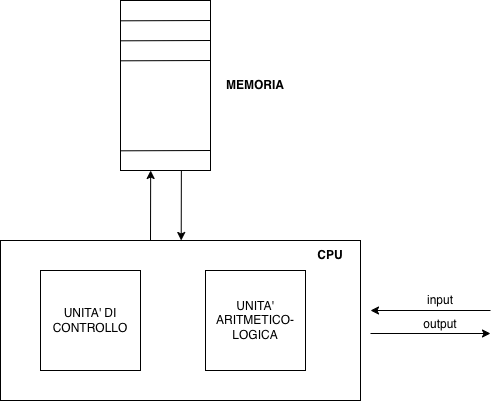
\includegraphics[width=0.5\textwidth]{images/arch-Von-Neumann}
      \caption{architettura di Von Neumann}
    \end{figure}

    Il linguaggio di programmazione, quindi, per poter operare su questa architettura, deve istruire una CPU per eseguire i calcoli (algoritmi) su dti conservati in memoria.

    \begin{figure}[H]
      \centering
      
\includegraphics[width=0.4\textwidth]{images/PL.png}
      \caption{lingauggio di programmazione}
    \end{figure}

    Da questa definizione, ne deriva che, anche il linguaggio binario è un lingauggio di programmazione, ma non è umanamente comprensibile perchè dati e istruzioni sono rappresentati nello stesso modo.\\[0.2ex]
   \hl{Un linguaggio di programmazione deve permttere di superare questa difficoltà}.

   \definition{algoritmo}{
    Un \textbf{algoritmo} è una sequenza passi, il cui scopo è il calcolo di una funzione.
   }

   Un algoritmo è un concetto astratto che trova forma concreta in un \textbf{programma}.

   \definition{programma}{
    Un \textbf{programma} è una sequenza (finita) di istruzioni.
   }

   \bigskip
   I \textcolor{verde}{\textbf{linguaggi di programmazione}} nascono, quindi, proprio per questo motivo: linguaggi formali le cui frasi sono programmi, ovvero forme concrete di algoritmi eseguibili/interpretabili da una macchina.


   \section{Cosa sono i linguaggi di programmazione}
   Il programma è la concretizzazione di un algoritmo che manipola i dati.\\[0.2ex]
   manca, però, un altro ingrediente: la \textbf{trasformazione} dei dati che l'algoritmo vuole eseguire.\\[0.2ex]
   \hl{Questa trasformazione è il significato dell'algoritmo, la semantica del programma}.
   \begin{itemize}[label=$\triangleright$]
    \item \textbf{programma}: costituisce la sintassi
    \smallskip
    \item \textbf{effetto dell'esecuzione del programma} (trasformazione dei dati): costituisce la semantica
   \end{itemize}

   \medskip
   Il programma è necessariamente un oggetto finito (sempre concreto), mentre il calcolo di una funzione richiede l'esecuzione di un insieme di passi primitivi, che però possono essere infiniti.\\[0.2ex]
   Questo significa che bisogna pensare al \hl{programma come a una rappresentazioen finita di un insieme potenzialmente inifinito, di passi primitivi di computazione}.

   \textbf{I linguaggi di programmazione devono dare specifica finita di oggetti potenzialmente infiniti}.
\end{document}